\documentclass[tikz, varwidth=6in]{standalone}

% arara: pdflatex: { interaction: batchmode }
% arara: latexmk: { clean: partial }
\begin{document}
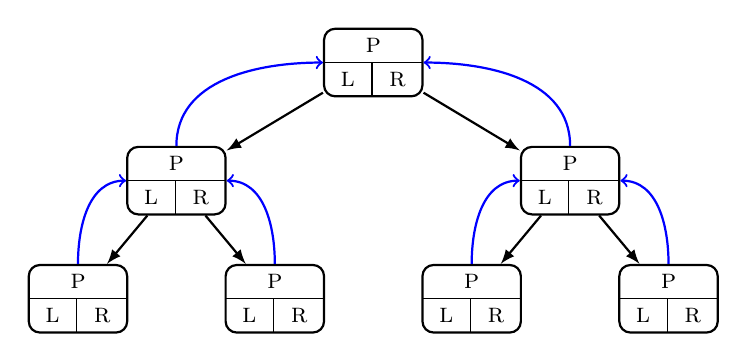
\begin{tikzpicture}[
	level distance=1.5cm,
	level 1/.style={sibling distance=5cm},
	level 2/.style={sibling distance=2.5cm},
	edge from parent/.style={draw,-latex},
	thick
]
\node[rounded corners, draw, inner sep=+0pt] (T){%
\begin{tabular}{c|c}
	\multicolumn{2}{c}{\textsc{p}} \\\hline
	\textsc{l} & \textsc{r}
	\end{tabular}}
	child { node[rounded corners, draw, inner sep=+0pt] (TL){%
		\begin{tabular}{c|c}
		\multicolumn{2}{c}{\textsc{p}} \\\hline
		\textsc{l} & \textsc{r}
		\end{tabular}}
		child { node[rounded corners, draw, inner sep=+0pt] (TLL){%
			\begin{tabular}{c|c}
			\multicolumn{2}{c}{\textsc{p}} \\\hline
			\textsc{l} & \textsc{r}
			\end{tabular}}
		}
		child { node[rounded corners, draw, inner sep=+0pt] (TLR){%
			\begin{tabular}{c|c}
			\multicolumn{2}{c}{\textsc{p}} \\\hline
			\textsc{l} & \textsc{r}
			\end{tabular}}
		}
	}
	child {node[rounded corners, draw, inner sep=+0pt] (TR) {%
		\begin{tabular}{c|c}
		\multicolumn{2}{c}{\textsc{p}} \\\hline
		\textsc{l} & \textsc{r}
		\end{tabular}}
		child { node[rounded corners, draw, inner sep=+0pt] (TRL){%
			\begin{tabular}{c|c}
			\multicolumn{2}{c}{\textsc{p}} \\\hline
			\textsc{l} & \textsc{r}
			\end{tabular}}
		}
		child { node[rounded corners, draw, inner sep=+0pt] (TRR){%
			\begin{tabular}{c|c}
			\multicolumn{2}{c}{\textsc{p}} \\\hline
			\textsc{l} & \textsc{r}
			\end{tabular}}
		}
	};
\draw[->,blue] (TL) to[out=90,in=180] (T);
\draw[->,blue] (TR) to[out=90,in=0] (T);
\draw[->,blue] (TRL) to[out=90,in=180] (TR);
\draw[->,blue] (TRR) to[out=90,in=0] (TR);
\draw[->,blue] (TLL) to[out=90,in=180] (TL);
\draw[->,blue] (TLR) to[out=90,in=0] (TL);
\end{tikzpicture}
\end{document}
